The fitter and background subtraction procedure, introduced in \Cref{sec:fitting_setup,sec:background_subtraction},
have been thoroughly validated in \Cref{sec:MC_validation} -- in simulation.
The real challenge, as usual, is ensuring that the conclusions and results observed in simulation will generalise correctly to real Belle II data.
The key concept of a blinded analysis dictates that one must validate the analysis procedure in control samples or regions -- collections of data that are abundant, well-understood and provide insight to the behaviour of signal in the detector.
In this Section, the discussion about \FEI validation, \piz and $\eta$ veto validation, photon detection efficiency and background modelling will be presented.

\subsection{Calibration of the \texorpdfstring{\FEI}{FEI} algorithm}\label{sec:fei_calibration}

The working principle of \FEI has already been discussed in XXXX
\todo[inline]{xxxx}.
It combines many classifiers which perform reconstructions in various decay chains of the hadronic decays of \B mesons.
Furthermore, the training of the algorithm happens in simulation.
To ensure that the algorithm appropriately acts on data, its performance on Belle II data must be studied, or \textit{calibrated}.
The calibration study is performed on data collected by the Belle~II, for every simulation campaign, and the work is not part of my original work.
Full details of the calibration method are presented in Ref.\cite{Belle-II:2020fst}, but here I will summarise the main details that are relevant to the work of the thesis.

The calibration study uses $B\rightarrow X_{u,c} \ell \nu$ decays, due to branching fraction of almost 20~\% and a clean experimental signature, 
where $X_{u,c}$ denotes an inclusive state originating from the $c$ or $u$ quark, similarly to the $X_s$ notation.
Firstly, in each event, only the highest \FEI probability tag-\B candidate is selected, with loose requirements on Fox-Wolfram moments (see \Cref{sec:fox_wolfram_moments}) and $\Delta E$ to ensure adequate \epem\ra\qqbar suppression.
Next, a high-energy lepton $p_{\ell}^B>1~\gev$ is required in each event.
This lepton candidate is required to originate near the interaction point and its identification information from all sub-detectors is required to be consistent with a lepton.

After the selection, a binned likelihood fit for \Mbc is set up, which contains three binned \PDF{s}: signal $B\rightarrow X_{u,c}\ell\nu$ decays, 
secondary or misidentified leptons, \epem\ra\qqbar events. Here secondary leptons are used to describe leptons that arise in the decay chains of $B$ meson as opposed to the $B\rightarrow X_{u,c}\ell\nu$ decay.
Misidentified leptons are used as a broad term for hadrons whose identification information is consistent with that of either an electron or a muon.
The signal $B\rightarrow X_{u,c}\ell\nu$ \PDF is composed of four sub-\PDF{s}, particularly: $B\rightarrow D\ell\nu$, $B\rightarrow D^*ell\nu$, $B\rightarrow X_u\ell\nu$ and the rest of  $B\rightarrow X_c\ell\nu$ modes.
The fit is performed separately for the following combinations of tag-\B mesons and lepton:
\begin{itemize}
    \item $B^+$ and $e^-$,
    \item $B^+$ and $\mu^-$,
    \item $B^0$ and $e^-$,
    \item $B^0$ and $\mu^-$.
\end{itemize}
This is shown in \Cref{fig:fei_calib}.
\begin{figure}[htbp!]
    \subcaptionbox{\label{fig:fei_calib_bpluseminus}}{
        \clipbox*{{0\width} {0.5\height} {0.5\width} {1\height}}{%
            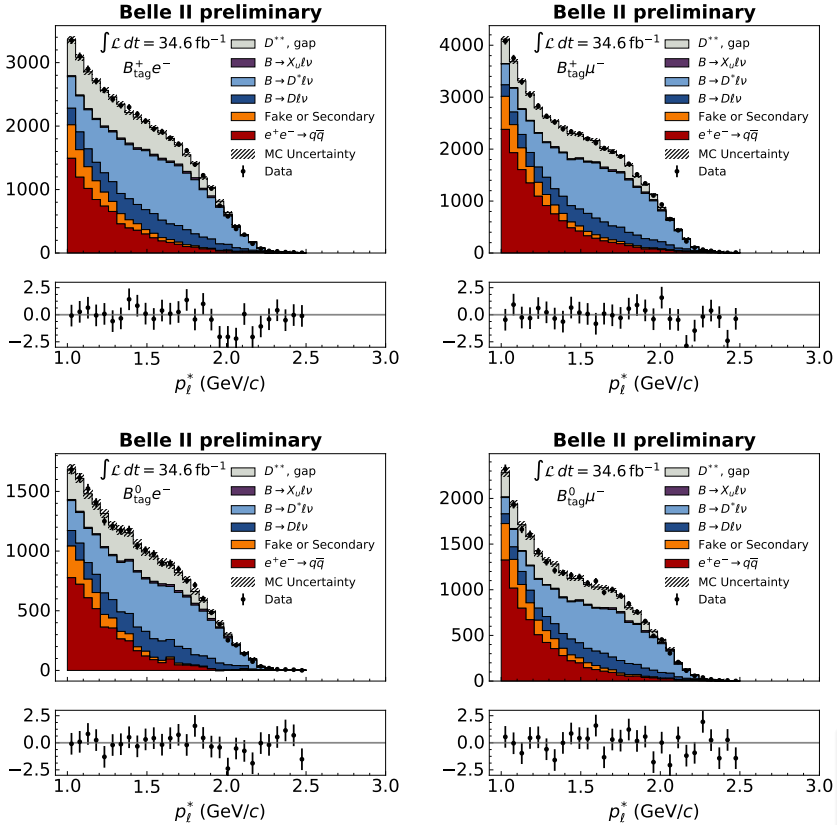
\includegraphics[width=1\textwidth]{figures/data_sim_corrections/tag_calibration.png}
        }
    }
    \subcaptionbox{\label{fig:fei_calib_bplusmuminus}}{
        \clipbox*{{0.5\width} {0.5\height} {1\width} {1\height}}{%
            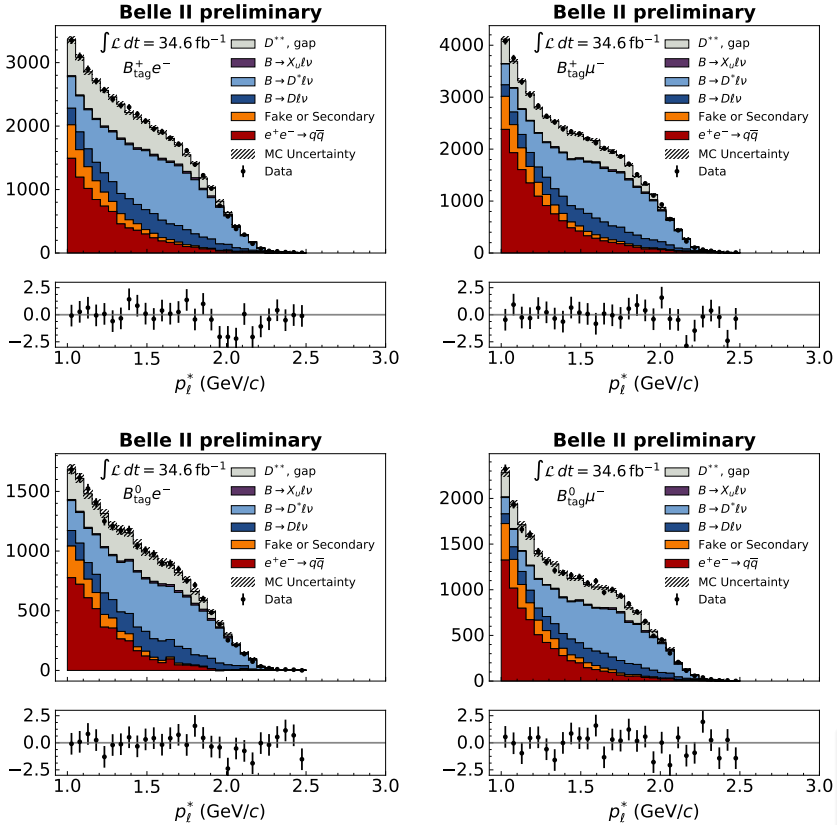
\includegraphics[width=1\textwidth]{figures/data_sim_corrections/tag_calibration.png}
        }
    }
    \subcaptionbox{\label{fig:fei_calib_bzeroeminus}}{
        \clipbox*{{0\width} {0\height} {0.5\width} {0.5\height}}{%
            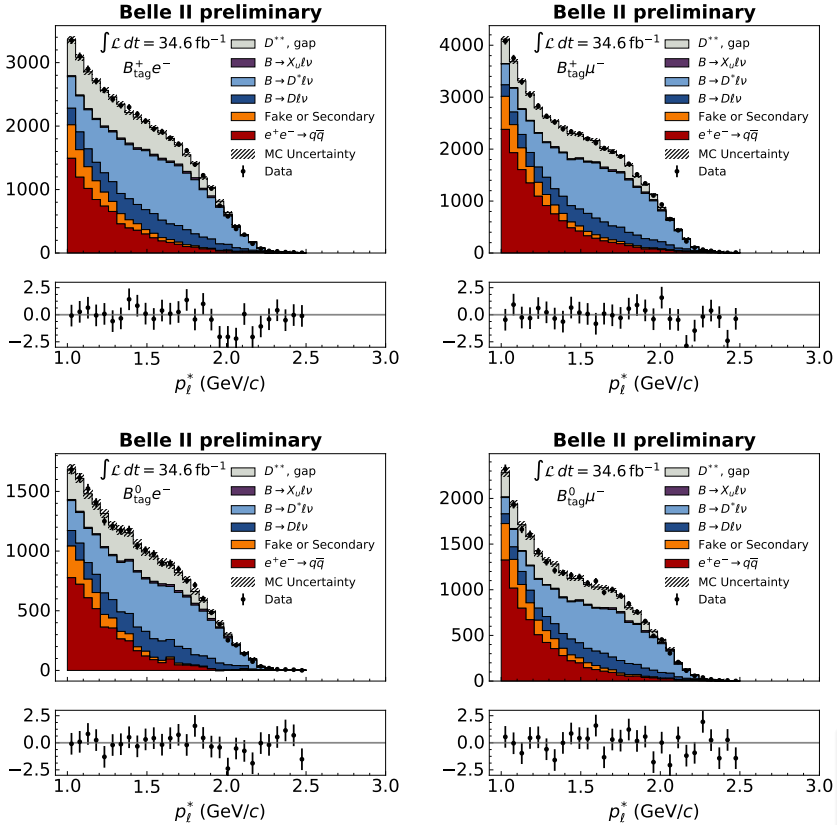
\includegraphics[width=1\textwidth]{figures/data_sim_corrections/tag_calibration.png}
        }
    }
    \subcaptionbox{\label{fig:fei_calib_bzeromuminus}}{
        \clipbox*{{0.5\width} {0\height} {1\width} {0.5\height}}{%
            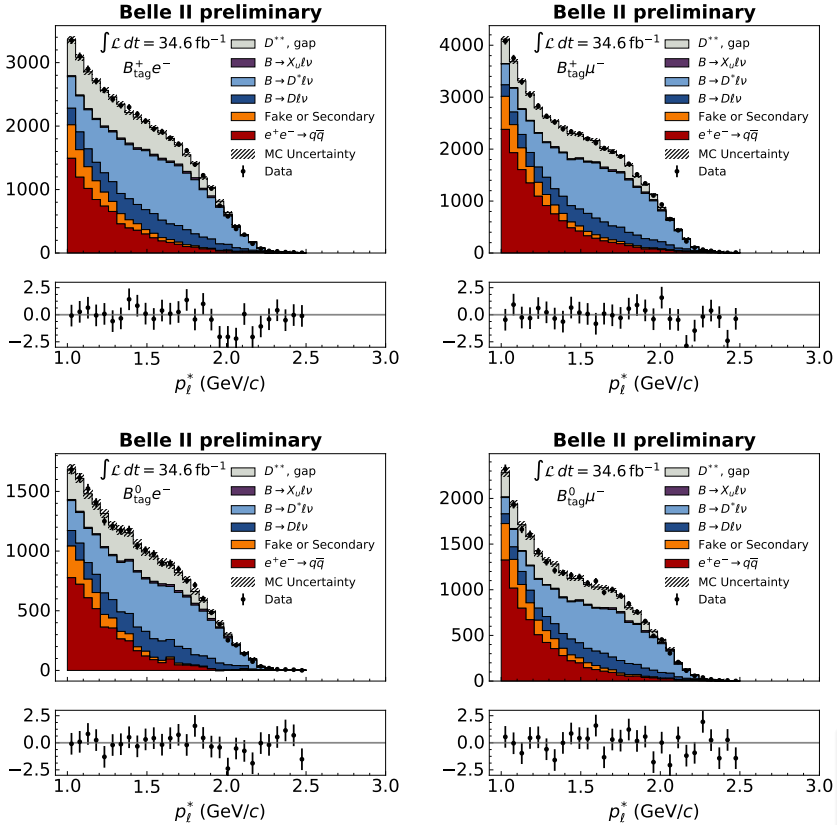
\includegraphics[width=1\textwidth]{figures/data_sim_corrections/tag_calibration.png}
        }
    }
    \caption{\label{fig:fei_calib} Illustration of the fits to \B\to$X_{u,c}\ell\nu$ decays in the \FEI calibration study.
    Results for the combinations of charged and neutral tag-$B$ modes with $e^-$ and $\mu^-$
    are shown in \Cref{fig:fei_calib_bpluseminus,fig:fei_calib_bplusmuminus,fig:fei_calib_bzeroeminus,fig:fei_calib_bzeromuminus}.
    Different fit components are shown in the legend and the subpanels contain the pulls of the fit.
    Figures taken from \cite{Belle-II:2020fst}.
    }
\end{figure}

Branching fractions of $B\rightarrow X_{u,c}\ell\nu$ are evaluated from the fitted distributions.
These values are then directly compared with the experimentally known values of branching fractions of these decays.
A correction factor, $\mathcal{C}_{\mathrm{FEI}}$ is derived, such that the two values are compatible.
The leading evaluated systematic uncertainties are found to be the imperfect experimental knowledge of the $B\rightarrow X_u\ell\nu$ branching fractions and their form factors, the fit model composition, tracking and particle identification uncertainties.
For the Belle II simulation campaign used in this analysis and averaged for both lepton modes, the result is as follows:
\begin{equation}\label{eq:fei_calibration}
    \mathcal{C}_{\mathrm{FEI}}(B^+) = 0.6599 \pm 0.225 \quad \mathcal{C}_{\mathrm{FEI}}(B^0) = 0.6695 \pm 0.0237,
\end{equation}
where two different calibration factors are presented for \feiBp and \feiBz modes, respectively.
Therefore, for an adequate comparison with Belle II data, any Belle II simulation involving the use of \FEI will be henceforth scaled appropriately.

\subsection{Calibration of \texorpdfstring{\piz}{pi0} and \texorpdfstring{$\eta$}{eta} suppression tools}\label{sec:piz_eta_calibration}
It was seen in \Cref{sec:selection_vetos}, that one of the strongest tools for background suppression in this analysis is the $\piz$ and $\eta$ suppression tool.
Consequentially, any data-simulation discrepancies will have a high impact on the final result.
The calibration of the \piz and $\eta$ is performed in an independent study and is not part of original work presented in this thesis.
For clarity, the calibration study is discussed in this Section.
\etaVeto calibration is henceforth implied, although only \piVeto is mentioned, as their calibration is equivalent.
Althrough the calibration study only studies \piVeto, it is assumed that the corrections are also valid for \etaVeto selections.

The main concern for this analysis is the primary (signal) photon efficiency: the number of photons that do not originate in light-meson decays and get rejected given a certain \piVeto selection.

The calibration study uses $B^+\to \bar{D}^0[\to K^+\pi^-]\pi^+$ decays and $B^0\to D^-[\to K^+\pi^-\pi^-]\pi^+$, where the square brackets denote a subdecay of the $D$ meson.
The $pi^+$, originating in the primary $B$ decay, is combined with all other photon candidates in the event, in a strategy described in \Cref{sec:selection_vetos}.
This produces many `\piz'-like combinations ($\mathit{pseudo-\piz}$) which yield a \piVeto score with minimal background from real \piz decays.

The reconstruction requires all charged tracks to have good-quality tracks that originate near the interaction point.
The identification information from Belle II subdetectors is used to distinguish pions and kaons.
Because $\pi^+$ from the primary $B$ decay is combined with other photons, a massless hypothesis is used for calculations of invariant mass and the helicity angles for the MVA.
After constructing the pseudo-\piz, selections on \piVeto are performed, corresponding to selections chosen in the analysis.
Therefore a distribution with no \piVeto selection, and a subset distribution with $\piVeto<0.4$ are created.
In both cases the charged and neutral $B$ channels are combined.

An unbinned \Mbc fit is performed on distributions with and without the \piVeto selections.
The \Mbc is modelled by a Crystal Ball function for signal decays and ARGUS function for continuum background.
All parameters of Crystal Ball and continuum are unconstrained.
An additional \PDF to model the peaking non-signal \BB components are used.
This \PDF is initialised in simulation, as a sum of a Gaussian and an Argus.
The shape parameters, and normalisation of this \BB background \PDF are not estimated, but kept at the initialised values.
The fits on data in the case of no \piVeto selection, and a $\piVeto<0.95$ selection are given in \Cref{fig:pivetofit}.
\begin{figure}[htbp!]
    \centering
    \subcaptionbox{\label{fig:pivetofit_nocut}}{
    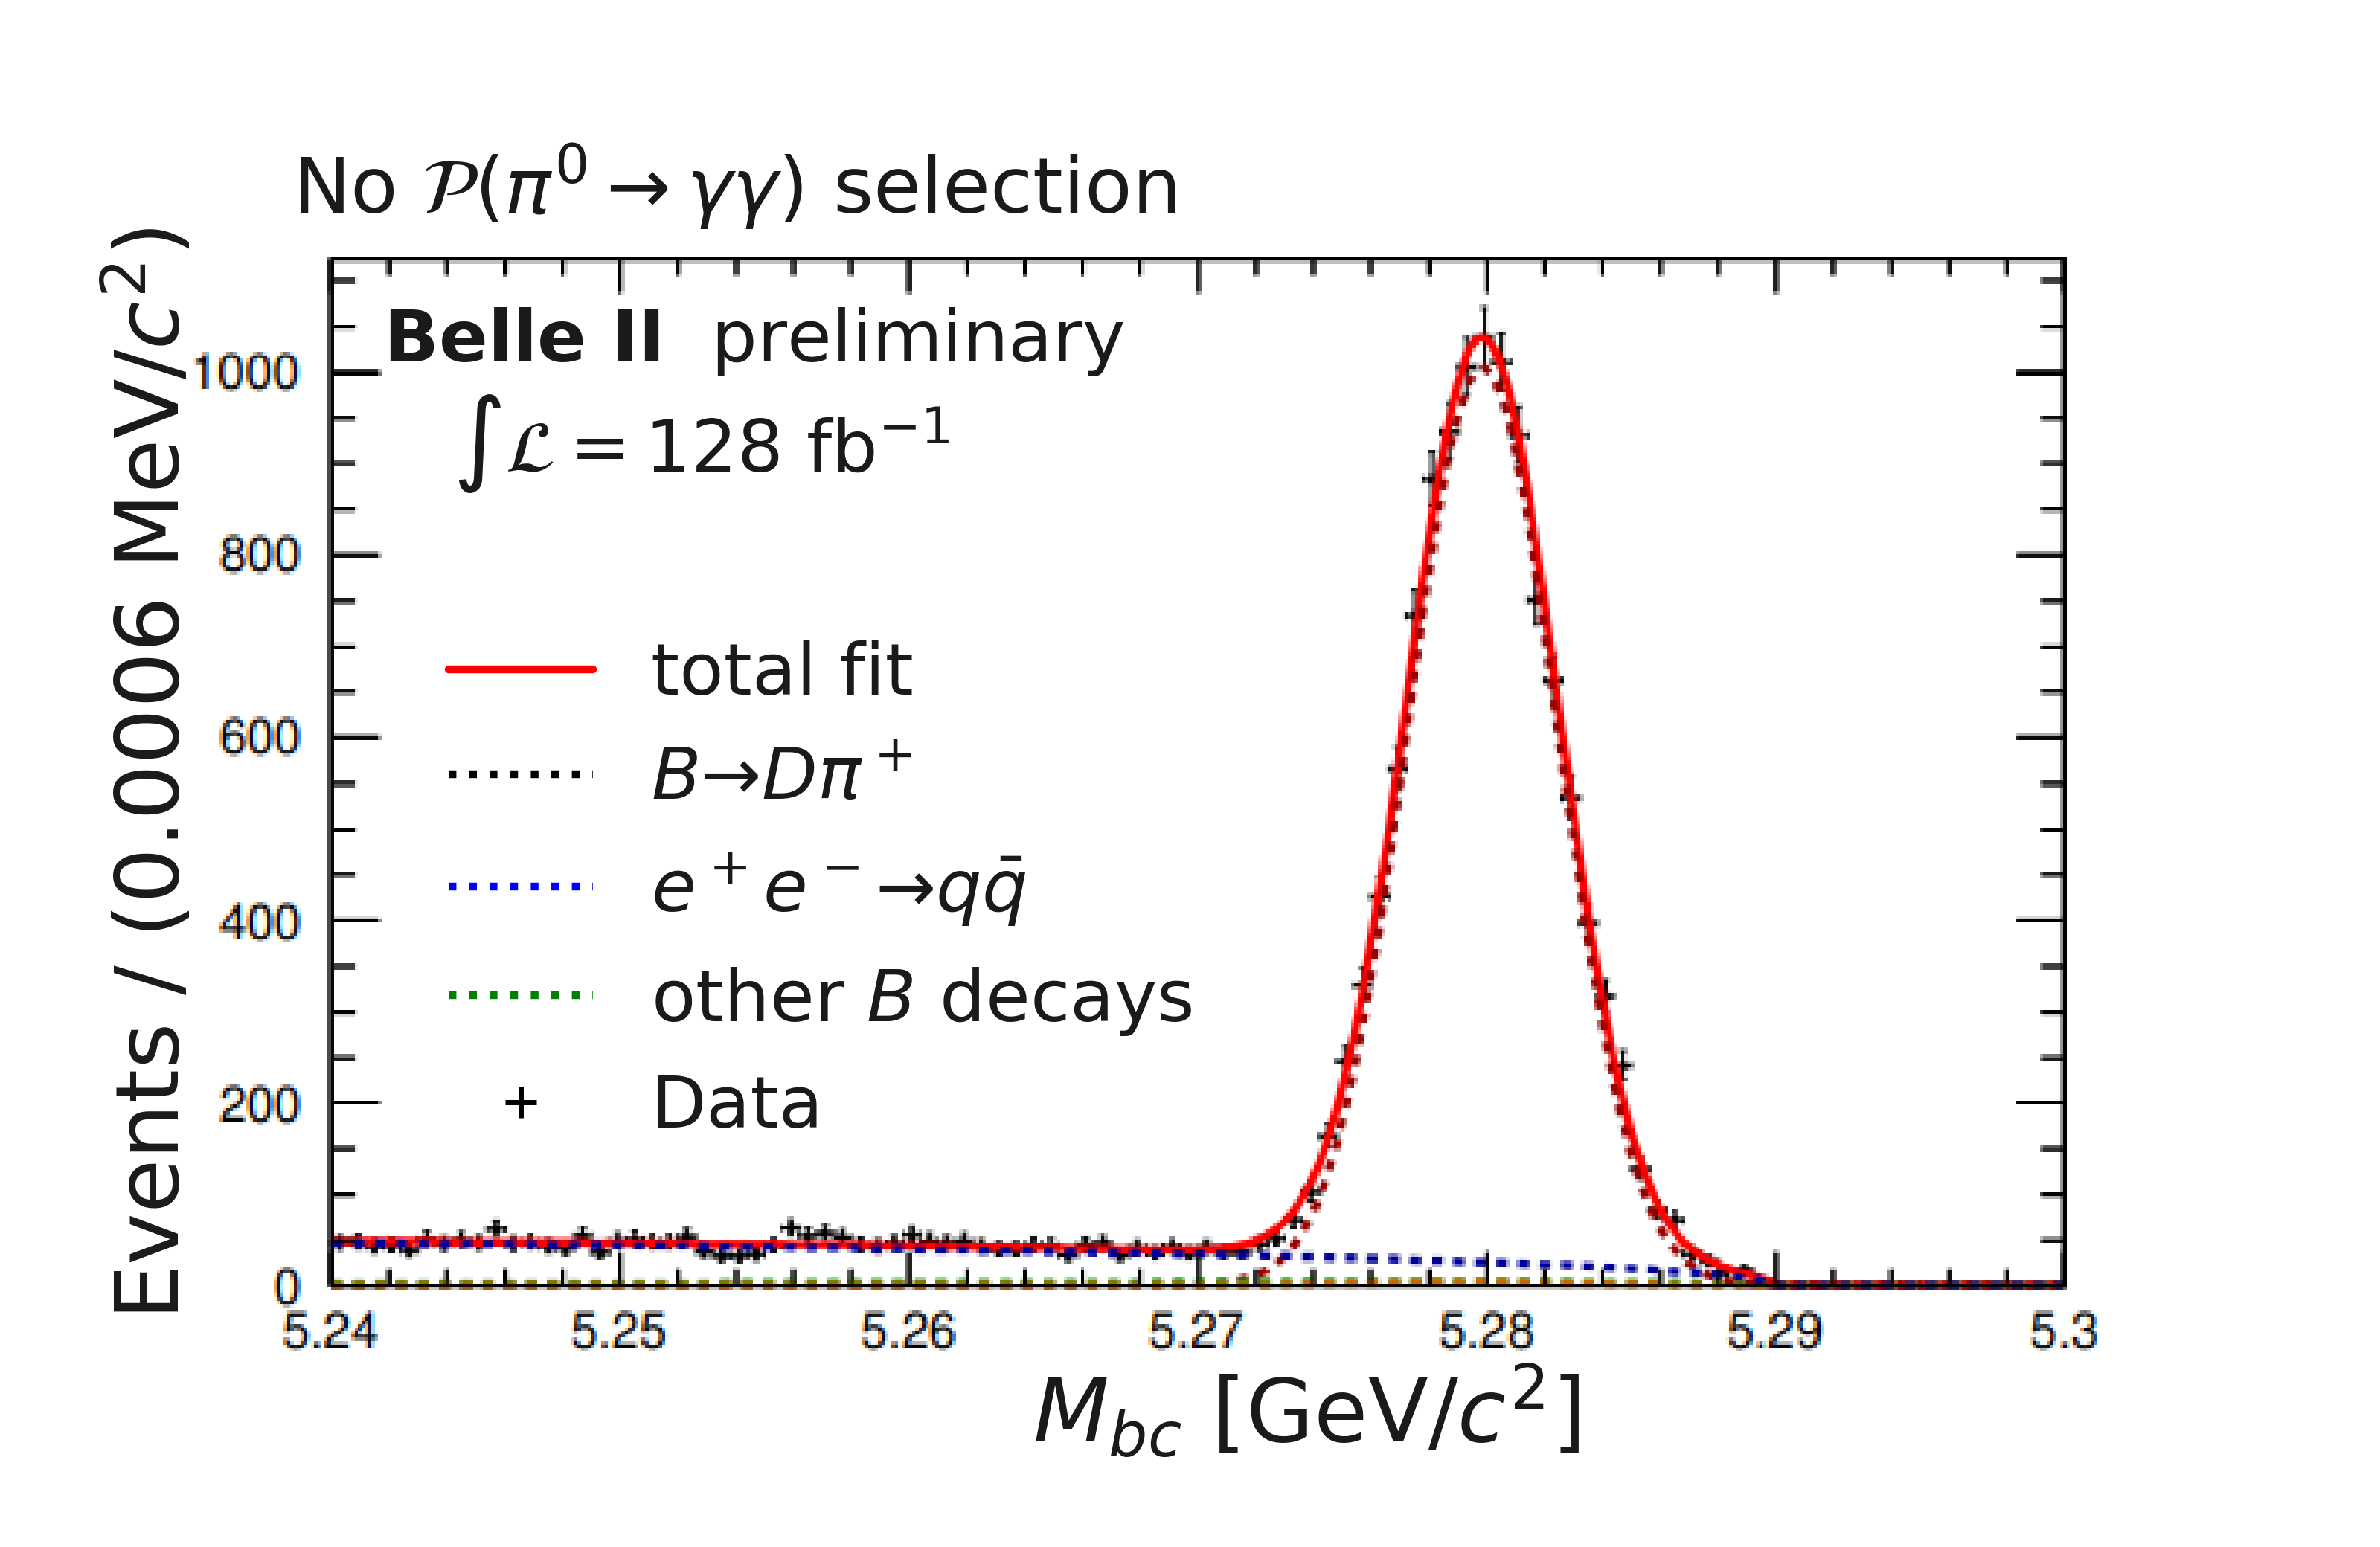
\includegraphics[width=0.4\textwidth]{figures/data_sim_corrections/data_fit_pi0_no_cut.png}
    }
    \subcaptionbox{\label{fig:pivetofit_cut}}{
        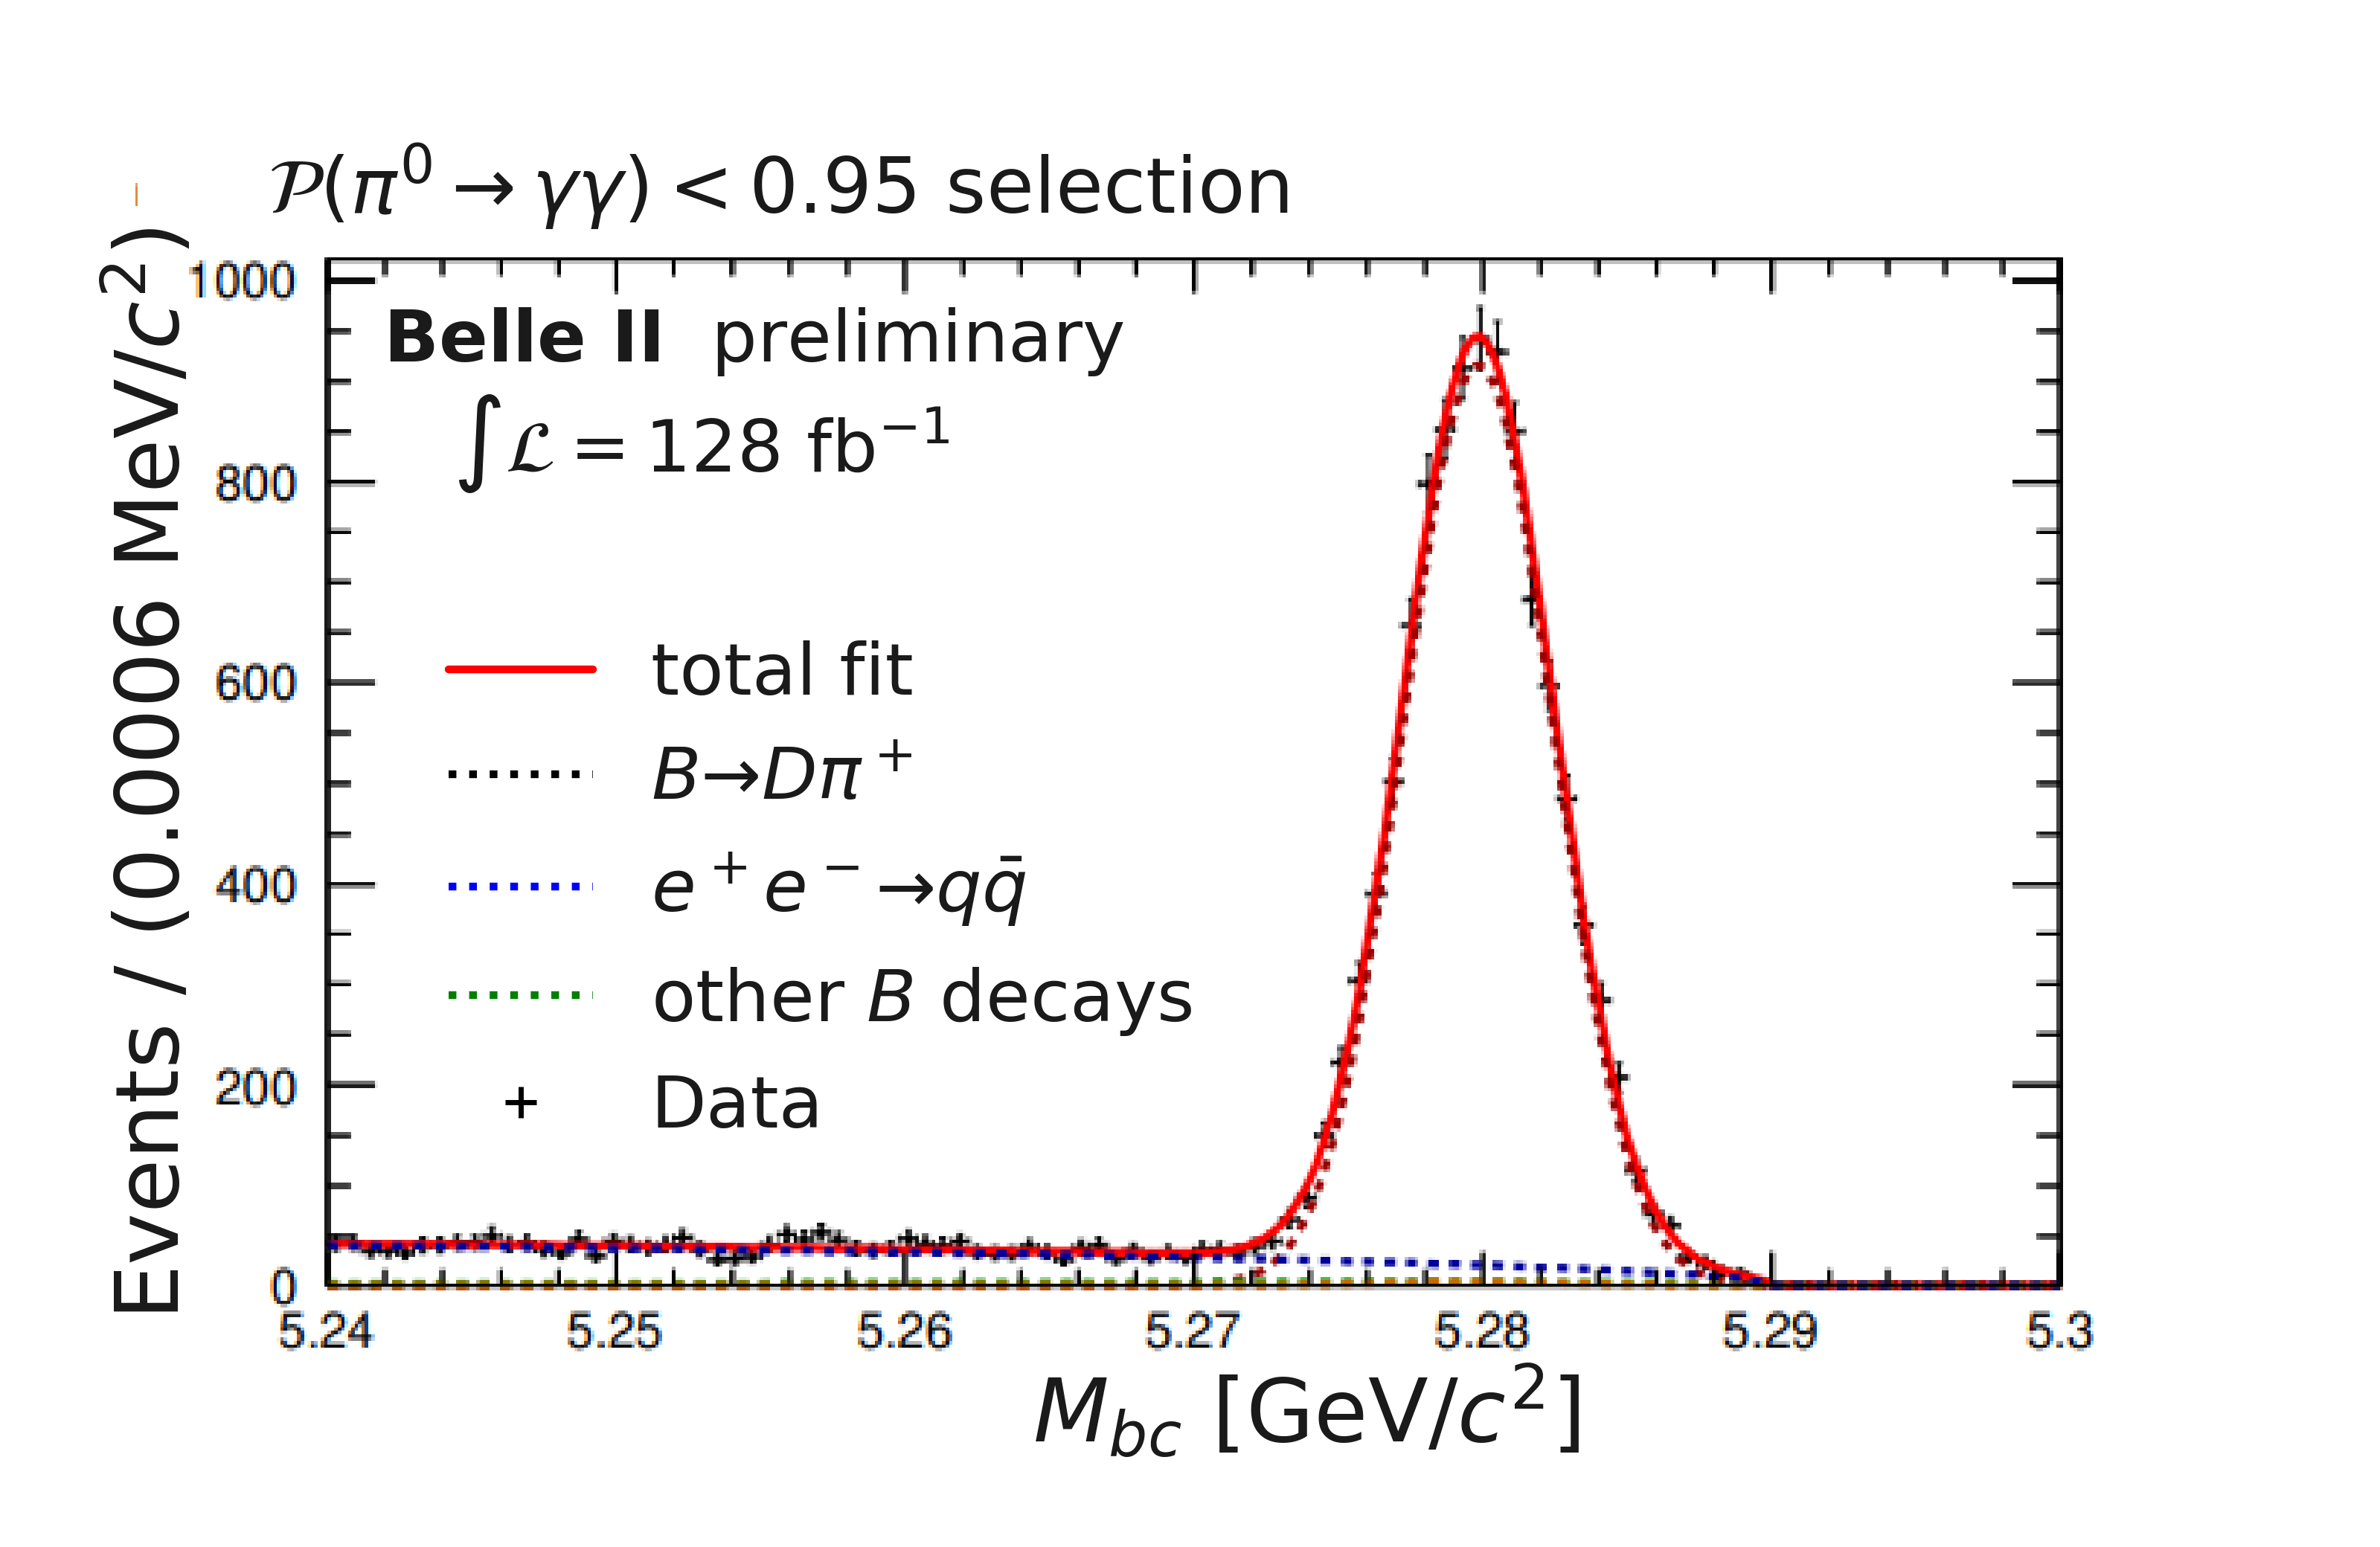
\includegraphics[width=0.4\textwidth]{figures/data_sim_corrections/data_fit_pi0_with_cut.png}
        }
    \caption{\label{fig:pivetofit} The fit estimating the number of $B\to D \pi^+$ events in Belle II data.
    Different \PDF{s} used in the fit are shown in the legend and explained in text.
    The fit is performed on a sample without (\Cref{fig:pivetofit_nocut}) and with (\Cref{fig:pivetofit_cut}) \piVeto selection applied.
    The extracted values from simulation and data are then combined to calculate \piVeto correction factors (see \Cref{eq:piveto_correction}).
    These figures are produced by a Belle II internal study of the \piz veto, and not part of the original work in this thesis.
    Only the labels and legends have been adapted.    
    }
\end{figure}

The fit extracts the counts of $B\to D\pi^+$ events, $N_{B\to D\pi^+}$ as the normalisation parameter of the Crystal Ball.
An efficiency, $\varepsilon\equiv N_{B\to D\pi^+}/N^{\piVeto<0.4}_{B\to D\pi^+}$ is defined, which corresponds to the primary-photon efficiency.
If the fit is performed in simulation (\MC) and data, an efficiency ratio can be used as a correction factor:
\begin{equation}\label{eq:piveto_correction}
    R_{\piVeto} = \frac{N_{B\to D\pi^+}/N^{\piVeto<0.4}_{B\to D\pi^+}|_{\mathrm{data}}}{N_{B\to D\pi^+}/N^{\piVeto<0.4}_{B\to D\pi^+}|_{\mathrm{MC}}}.
\end{equation}
The corrections are calculated in $200~\mev$ intervals of the lab-frame energy of the primary $\pi^+$.
The results for the selection chosen in this analysis are given in \Cref{fig:piveto_corrections}.
The internal Belle II study providing these corrections was only performed in the range of 1.8 to 3.0 ~\gev in the laboratory frame energy of the primary $\pi^+$.
Therefore, a linear extrapolation based is performed to estimate the value for values outside the range.
It is observed that the linear extrapolation is consisttent, within errors, with the corrections in the $1.8-3.0~\gev$.
Therefore, a correction factor of $1.1\pm0.5$ is chosen for events outside the range covered by the calubration study.
This value is consistent with all other correction factors.
\begin{figure}[htbp!]
    \centering
    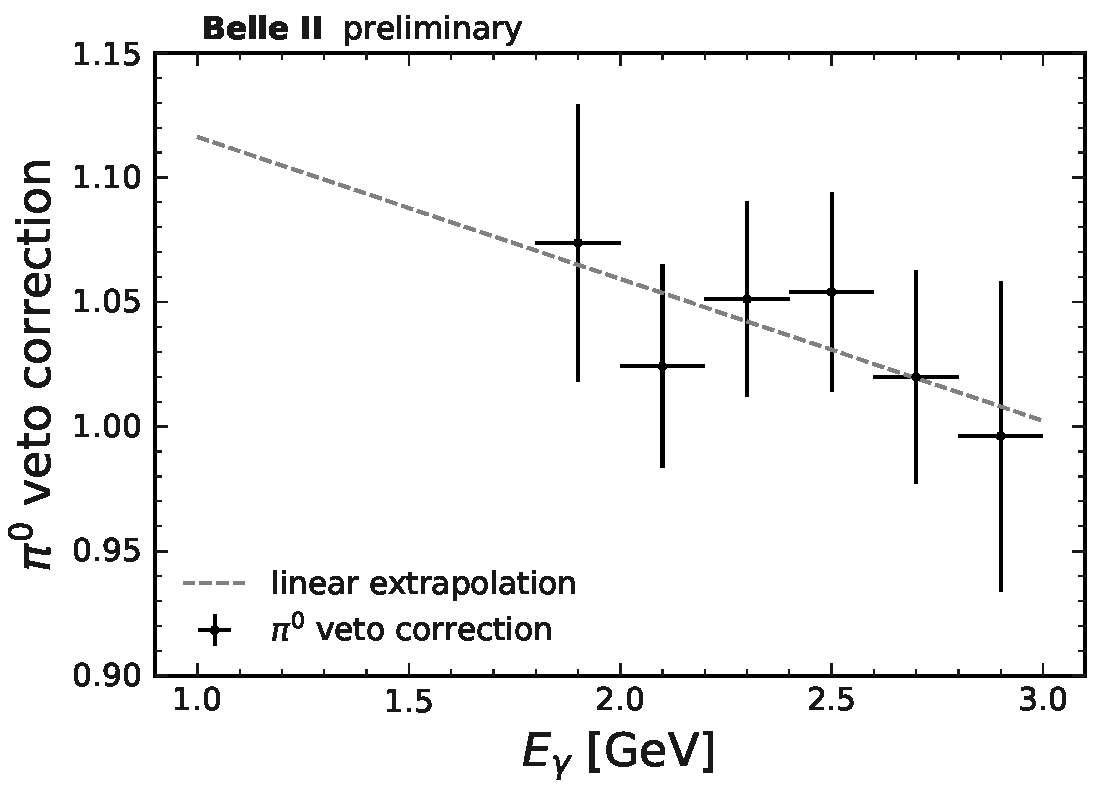
\includegraphics[width=0.45\textwidth]{figures/data_sim_corrections/pi0veto_corrections.pdf}
    \caption{\label{fig:piveto_corrections} The corrections $R_{\piVeto}$ for the $\piVeto<0.4$ selection used in this analysis.
    The results cover $1.8-3.0~\gev$ energies in the \textit{laboratory frame}, $\Egamma$.
    Because the laboratory frame energies cannot be trivially transformed to the $B$ meson rest-frame energies, a linear extrapolation to lower energies is performed.
    For missing $\Egamma$ phase space, in this analysis a $1.1\pm0.5$ value is adopted.
    }
\end{figure}

\subsection{Belle II calorimeter photon detection efficieny}\label{sec:photon_efficiency}

